This chapter surveys the research areas on which this thesis builds. We first review deep clustering and its dominant single-algorithm paradigm (Section~\ref{sec:rw_deep}), then consensus clustering and the DECCS framework that motivates our robustness goal (Section~\ref{sec:rw_consensus}). We then turn to explainable and descriptive clustering, including the DDC framework that motivates our interpretability goal (Section~\ref{sec:rw_explainable}). Finally, we position our work against the gap that none of these methods fill, including the one prior approach that, like ours, targets interpretable consensus clustering (Section~\ref{sec:rw_gap}).

\section{Deep Clustering}
\label{sec:rw_deep}

Deep clustering jointly learns a feature representation and a cluster assignment, replacing the hand-crafted features used by classical algorithms. Deep Embedded Clustering (DEC)~\citep{Xie2016} is the seminal method: it pre-trains a stacked autoencoder, then refines the embedding by minimizing the Kullback--Leibler divergence between soft cluster assignments and a sharpened target distribution. DEC established the template of alternating between representation learning and cluster refinement that most later methods follow.

Subsequent work extended DEC along several directions. Improved DEC (IDEC)~\citep{Guo2017} retains the autoencoder's reconstruction term during clustering to preserve local structure. Deep Adaptive Clustering (DAC)~\citep{Chang2017} reformulates image clustering as a binary pairwise-classification problem. JULE~\citep{Yang2016} jointly learns representations and assignments in a recurrent agglomerative framework, and DeepCluster~\citep{Caron2018} alternates between k-means on learned features and using the resulting assignments as pseudo-labels. Deep embedded cluster trees~\citep{Mautz2020} extend the paradigm to hierarchical clustering. Comprehensive surveys of the field are provided by~\citet{Min2018} and~\citet{Zhou2024}.

The common limitation across these methods is twofold. First, each is tied to a \emph{single} clustering objective---typically k-means-style or spectral---so its quality depends on how well that objective's assumptions match the data. Second, the learned representations are opaque: they yield cluster assignments but no human-readable account of what distinguishes one cluster from another. The two families of work we review next address these two limitations independently.

\section{Consensus Clustering}
\label{sec:rw_consensus}

Consensus (or ensemble) clustering improves robustness by combining several clusterings into a single partition, so that the result does not depend on any one algorithm's assumptions. Classical consensus methods build a co-association matrix from multiple base partitions and then re-cluster it~\citep{Strehl2002, Fred2005}; broader surveys are given by~\citet{Vega-Pons2011}. Their main limitation is that they operate on fixed input features or on the partitions alone, and are typically restricted to linear relationships---they do not learn a new representation from the raw data.

Deep Clustering with Consensus Representations (DECCS)~\citep{Miklautz2022} removes this limitation by learning a non-linear consensus representation with an autoencoder. The encoder is trained so that a heterogeneous ensemble of clustering algorithms (for example k-means, spectral clustering, and Gaussian mixtures) increasingly \emph{agree} with one another when applied to the embedded data. Concretely, the encoder parameters $\Theta$ are optimized to maximize the average pairwise agreement of the ensemble members,
\[
    f_{\Theta} = c \sum_{i=1}^{|\mathcal{E}|} \sum_{j>i}^{|\mathcal{E}|} \mathrm{NMI}\!\left(e_i(\mathrm{enc}_{\Theta}(X)),\, e_j(\mathrm{enc}_{\Theta}(X))\right),
\]
where $X$ is the input data, $\mathrm{enc}_{\Theta}$ is the encoder, $\mathcal{E} = \{e_1, \ldots\}$ is the set of clustering algorithms, $\mathrm{NMI}$ is the normalized mutual information between two clusterings, and $c = 2 / (|\mathcal{E}|^2 - |\mathcal{E}|)$ normalizes the sum to one. One round of DECCS, illustrated in Figure~\ref{fig:deccs}, embeds the data, applies the ensemble, trains classifiers to predict each member's assignments, and updates the encoder to increase agreement.

\begin{figure}[H]
    \centering
    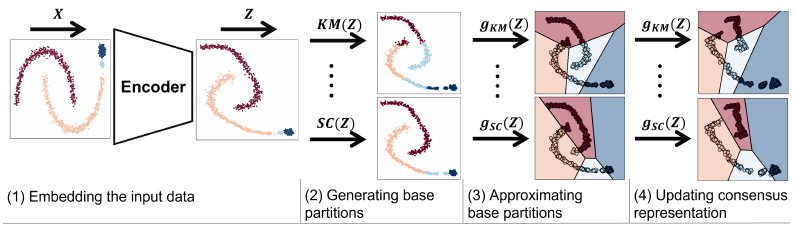
\includegraphics[width=\textwidth]{figs/deccs.png}
    \caption{One round of DECCS~\citep{Miklautz2022}. (1) The encoder embeds data points $X$. (2) Clusterings are generated by applying ensemble members $\mathcal{E}$ to the embedding $Z$. (3) Classifiers $g_i$ are trained to predict the cluster labels $\pi_i$ from $Z$. (4) $Z$ is updated by minimizing the loss $\mathcal{L}$.}
    \label{fig:deccs}
\end{figure}

The strength of DECCS is robustness: by maximizing agreement across diverse algorithms, it learns representations that are stable and reproducible rather than dependent on a single algorithm's inductive bias. Its limitation, for our purposes, is that the consensus is purely statistical---it produces no explanation of why instances are grouped together, and the learned representation has no semantic grounding.

\section{Explainable and Descriptive Clustering}
\label{sec:rw_explainable}

Explainable clustering methods fall into two broad families. \emph{Explainable-by-design} methods~\citep{Bertsimas2020, Moshkovitz2020} build the clustering directly from interpretable features, for example by constructing a small decision tree whose splits both define and explain the clusters. Their strength is that the explanation is exact and intrinsic; their weakness is that they require interpretable input features, which rules out complex data such as images whose raw pixels are not meaningful to a human.

\emph{Post-processing} methods~\citep{davidson2018, Sambaturu2020} instead take an existing clustering and attach explanations after the fact, typically using a separate set of semantic tags. They are algorithm-agnostic and can therefore explain the output of any clustering method, but because the explanation step is decoupled from clustering, the quality of the explanation depends entirely on how well the original clustering happens to align with the available tags. Instance-level methods such as LIME~\citep{Ribeiro2016} explain individual predictions with local surrogate models but do not characterize entire clusters.

Deep Descriptive Clustering (DDC)~\citep{Zhang2021} bridges these families for complex data. DDC clusters by maximizing the mutual information between the inputs and the induced cluster labels, and simultaneously generates a cluster-level explanation by solving an Integer Linear Programming (ILP) problem that selects, for each cluster, a small set of semantic attributes. The ILP enforces \emph{orthogonality} through an upper bound on how much each attribute's coverage may be shared across clusters, so that the descriptions for different clusters stay concise and minimally overlapping. A self-generated pairwise loss then feeds the explanation back into the clustering objective, encouraging the two modules to agree. The framework is illustrated in Figure~\ref{fig:ddc}.

\begin{figure}[H]
    \centering
    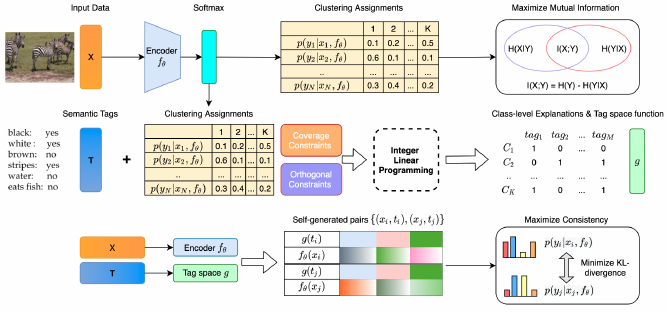
\includegraphics[width=\textwidth]{figs/ddc.png}
    \caption{The DDC framework~\citep{Zhang2021}, comprising a clustering objective (mutual information maximization), a symbolic explanation objective (ILP-based tag selection), and a self-generated pairwise objective that maximizes consistency between the clustering and explanation modules.}
    \label{fig:ddc}
\end{figure}

The strength of DDC is interpretability: it is, to our knowledge, the first deep clustering method to produce concise, orthogonal cluster-level descriptions for complex image data. Its limitation, for our purposes, is that it relies on a single clustering objective and therefore does not benefit from the robustness that an ensemble provides.

\section{Summary and Research Gap}
\label{sec:rw_gap}

Table~\ref{tab:qualitative_comparison} summarizes the capabilities of the methods reviewed above. Two observations stand out. Consensus clustering (DECCS) delivers robustness but no interpretability, while descriptive clustering (DDC) delivers interpretability but uses a single clustering algorithm. No prior method provides both ensemble-based robustness and semantic cluster descriptions for complex image data.

\begin{table}[H]
    \centering
    \caption{Capability comparison of the clustering methods reviewed in this chapter. DDECCS denotes the framework proposed in this thesis.}
    \label{tab:qualitative_comparison}
    \begin{tabular}{lcccc}
        \hline
        \textbf{Capability} & \textbf{DEC} & \textbf{DECCS} & \textbf{DDC} & \textbf{DDECCS} \\
        \hline
        Ensemble / consensus clustering & \xmark & \cmark & \xmark & \cmark \\
        Uses semantic attributes        & \xmark & \xmark & \cmark & \cmark \\
        Cluster-level descriptions       & \xmark & \xmark & \cmark & \cmark \\
        Handles complex (image) data     & \cmark & \cmark & \cmark & \cmark \\
        Interpretable input required     & \xmark & \xmark & \xmark & \xmark \\
        \hline
    \end{tabular}
\end{table}

DDECCS targets exactly this gap, combining DECCS-style consensus with DDC-style descriptions so that the final clusters are both robust and interpretable. The next chapter develops the pipeline in detail.